\documentclass{article}
\usepackage{graphicx}
\usepackage{IEEEtrantools}
\usepackage{amsmath}

\title{Solve $Z_1 = Z_2$ for $x_1$}
\author{Daniel Fishbein}

\begin{document}
\maketitle

\section{Given:}

\begin{figure}[h!]{
    \centering
    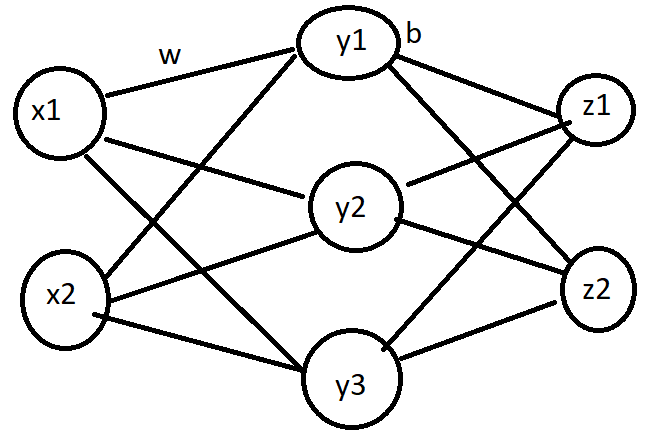
\includegraphics[width=0.5\linewidth]{Given_NN.png}
    \caption{Given Neural Net}\label{fig:NeuralNet}
    }
\end{figure}

\hbox{Figure~\ref{fig:NeuralNet} shows the given Neural Net that will be analysed.}

\vspace{5mm}

\hbox{$x_1, x_2$ are the input neurons}
\hbox{$[x]$ is the columnised vector notation of all "x" neurons of dimentions $1$X$x$}
\vspace{1mm}

\hbox{$y_1, y_2, y_3$ are the hidden layers neurons}
\hbox{$[y]$ is the columnised vector notation of all "y" neurons of dimentions $1$X$y$}
\vspace{1mm}

\hbox{$z_1, z_2$ are the output neurons}
\hbox{$[z]$ is the columnised vector notation of all "z" neurons of dimentions $1$X$z$}

\vspace{2mm}
\hbox{$w$ denotes a weight}
\hbox{$w_{y_1->z_2}$ denotes the weight from $y_1$ to $z_2$}
\hbox{$[w_1]$ is the columnised vector notation of all "$w_1$" weights of dimentions $y$X$x$}
\hbox{$[w_1] = [
    \begin{matrix}
        w_{11} w_{12} w_{13} ... w_{1x} \\
        :\\
        w_{ij}\\
        :\\
        w_{y1} w_{y2} w_{y3} ... w_{yx}
    \end{matrix}
]$}

\vspace{2mm}
\hbox{$[w_2]$ is the columnised vector notation of all "$w_2$" weights of dimentions $z$X$y$}
\hbox{$[w_2] = [
    \begin{matrix}
        w_{11} w_{12} w_{13} ... w_{1y} \\
        :\\
        w_{ij}\\
        :\\
        w_{z1} w_{z2} w_{z3} ... w_{zy}
    \end{matrix}
]$}


\vspace{4mm}
\hbox{$b$ deontes a bias}
\hbox{$b_{y_3}$ deontes the bias associated with neuron $y_3$}
\hbox{$[b_1]$ is the columnised vector notation of all "$b_1$" biases of dimentions $1$X$y$ }
\hbox{$[b_1] = [
    \begin{matrix}
        b_{11}\\
        b_{21}\\
        :\\
        b_{1y}
    \end{matrix}
]$}

\vspace{2mm}
\hbox{$[b_2]$ is the columnised vector notation of all "$b_2$" biases of dimentions $1$X$z$ }
\hbox{$[b_2] = [
    \begin{matrix}
        b_{11}\\
        b_{21}\\
        :\\
        b_{1z}
    \end{matrix}
]$}

\vspace{5mm}
\hbox{The input to a $y_i$ neuron will be denoted as:}
\hbox{$y_i = \sigma(w_{x_1->y_i} * x_1 + w_{x_2->y_i} * x_2 + b_{y_i} )$}
\hbox{OR in vector notation:}
\hbox{$[y] = \sigma([x][w_1] + [b_1])$}

\vspace{2mm}
\hbox{Where $\sigma(x) = \frac{1}{1+e^{-x}} = \frac{1}{1+\exp[-x]}$}

\vspace{5mm}
\hbox{The input to a $z_i$ neuron will be denoted as:}
\hbox{$z_i = \sigma(w_{y_1->z_i}*y_1 + w_{y_2->z_i}*y_2 + w_{y_3->z_i}*y_3 + b_{z_i} )$}
\hbox{OR in vector notation:}
\hbox{$[z] = \sigma([y][w_2] + [b_2])$}





\section{Solve $z_1 = z_2$ for $x_1$}
\begin{equation}
    z_1 = z_2    
\end{equation}

\hbox{NOTE: Observe I as the identity matrix}

\begin{equation}
    I = \begin{bmatrix}
        1 & 0 & 0\\
        0 & 1 & 0\\
        0 & 0 & 1\\
    \end{bmatrix}
\end{equation}

\hbox{NOTE: Observe $[x]I$}
\[
[x]I = \begin{bmatrix}   
    x_1\\
    x_2\\
    x_3\\
    \end{bmatrix}
%
\begin{bmatrix}   
    1 & 0 & 0 \\
    0 & 1 & 0 \\
    0 & 0 & 1 \\
    \end{bmatrix} = 
%
    \begin{bmatrix}
        x_1\\
        x_2\\
        x_3\\
    \end{bmatrix}
\]

\hbox{NOTE: Observe:}
\[
\begin{bmatrix}   
    x_1\\
    x_2\\
    x_3\\
    \end{bmatrix}
%
\begin{bmatrix}   
    1 & 0 & 0 \\
    0 & 0 & 0 \\
    0 & 0 & 0 \\
    \end{bmatrix} = 
%
    \begin{bmatrix}
        x_1\\
        0\\
        0\\
    \end{bmatrix}
\]

\[
\begin{bmatrix}   
    x_1\\
    x_2\\
    x_3\\
    \end{bmatrix}
%
\begin{bmatrix}   
    0 & 0 & 0 \\
    0 & 1 & 0 \\
    0 & 0 & 0 \\
    \end{bmatrix} = 
%
    \begin{bmatrix}
        0\\
        x_2\\
        0\\
    \end{bmatrix}
\]

\hbox{Denote:}

\[
    [I_1] = \begin{bmatrix}   
    1 & 0 & 0 \\
    0 & 0 & 0 \\
    0 & 0 & 0 \\
    \end{bmatrix}
\]

\hbox{Denote:}

\[
    [I_2] = \begin{bmatrix}   
    0 & 0 & 0 \\
    0 & 1 & 0 \\
    0 & 0 & 0 \\
    \end{bmatrix}
\]

\hbox{we can rewrite: $z_1 = z_2$ as:}

\begin{equation}
    [z][I_1] = [z][I_2]
\end{equation}

\hbox{move everything to one side}
\begin{equation}
    [z][I_1] - [z][I_2] = 0
\end{equation}


\hbox{factor $[z]$}
\begin{equation}
    [z]([I_1] - [I_2]) = 0
\end{equation}

\hbox{expand $[I_1]$ and $[I_2]$}
\begin{equation}
    [z](\begin{bmatrix}   
        1 & 0 & 0 \\
        0 & 0 & 0 \\
        0 & 0 & 0 \\
        \end{bmatrix} 
        - 
        \begin{bmatrix}   
            0 & 0 & 0 \\
            0 & 1 & 0 \\
            0 & 0 & 0 \\
            \end{bmatrix}) = 0
\end{equation}

\hbox{simplify}
\begin{equation}
    [z]\begin{bmatrix}   
        1 & 0 & 0 \\
        0 & -1 & 0 \\
        0 & 0 & 0 \\
        \end{bmatrix} = 0
\end{equation}

\hbox{Denote: }
\begin{equation}
    [I_{1-2}] = \begin{bmatrix}   
        1 & 0 & 0 \\
        0 & -1 & 0 \\
        0 & 0 & 0 \\
        \end{bmatrix}
\end{equation}

\hbox{return to matrix notation}
\begin{equation}
    [z][I_{1-2}] = 0
\end{equation}


\hbox{expand $[z]$}

\begin{equation}
    [z] = \sigma([y][w_2] + [b_2])
\end{equation}

\begin{equation}
    [z] = \sigma(
            \sigma([x][w_1] + [b_1])
        [w_2] + [b_2])
\end{equation}

\hbox{substatute eq.11 into eq.9}

\begin{equation}
    \sigma(
            \sigma([x][w_1] + [b_1])
        [w_2] + [b_2])[I_{1-2}] = 0
\end{equation}

\hbox{expand out matricies}


\[
\theta(
    \theta(
\begin{bmatrix}   
    x_1\\
    x_2\\
    x_3\\
    \end{bmatrix}
    %
\begin{bmatrix}
    w_{y11} & w_{y12} & w_{y13}\\
    w_{y21} & w_{y22} & w_{y23}\\
    w_{y31} & w_{y32} & w_{y33}\\
\end{bmatrix}
    +
\begin{bmatrix}
    b_{y1}\\
    b_{y2}\\
    b_{y3}\\
\end{bmatrix}
    )
    %
\begin{bmatrix}
    w_{z11} & w_{z12} & w_{z13}\\
    w_{z21} & w_{z22} & w_{z23}\\
    w_{z31} & w_{z32} & w_{z33}\\
\end{bmatrix}
    +
\begin{bmatrix}
    b_{z1}\\
    b_{z2}\\
    b_{z3}\\
\end{bmatrix}
)
%
\begin{bmatrix}   
    1 & 0 & 0 \\
    0 & -1 & 0 \\
    0 & 0 & 0 \\
    \end{bmatrix} 
%
    = 0
\]
\hbox{NOTE: will need the transpos of $[x]$}

\[
\theta(
    \theta(
\begin{bmatrix}   
    x_1 & x_2  & x_3\\
    \end{bmatrix}
    %
\begin{bmatrix}
    w_{y11} & w_{y12} & w_{y13}\\
    w_{y21} & w_{y22} & w_{y23}\\
    w_{y31} & w_{y32} & w_{y33}\\
\end{bmatrix}
    +
    \begin{bmatrix}
        b_{y1}\\
        b_{y2}\\
        b_{y3}\\
    \end{bmatrix}
    )
    %
\begin{bmatrix}
    w_{z11} & w_{z12} & w_{z13}\\
    w_{z21} & w_{z22} & w_{z23}\\
    w_{z31} & w_{z32} & w_{z33}\\
\end{bmatrix}
    +
    \begin{bmatrix}
        b_{z1}\\
        b_{z2}\\
        b_{z3}\\
    \end{bmatrix}
)
%
\begin{bmatrix}   
    1 & 0 & 0 \\
    0 & -1 & 0 \\
    0 & 0 & 0 \\
    \end{bmatrix} 
%
    = 0
\]

\hbox{simplify}

\[
\theta(
    \theta(
\begin{bmatrix}   
    x_1*w_{y11} + x_2*w_{y21} + x_3*w_{y31}\\
    x_1*w_{y12} + x_2*w_{y22} + x_3*w_{y32}\\
    x_1*w_{y13} + x_2*w_{y23} + x_3*w_{y33}\\
    \end{bmatrix}
    +
    \begin{bmatrix}
        b_{y1}\\
        b_{y2}\\
        b_{y3}\\
    \end{bmatrix}
    )
    %
\begin{bmatrix}
    w_{z11} & w_{z12} & w_{z13}\\
    w_{z21} & w_{z22} & w_{z23}\\
    w_{z31} & w_{z32} & w_{z33}\\
\end{bmatrix}
    +
\begin{bmatrix}
    \begin{bmatrix}
        b_{z1}\\
        b_{z2}\\
        b_{z3}\\
    \end{bmatrix}
\end{bmatrix}
)
%
\begin{bmatrix}   
    1 & 0 & 0 \\
    0 & -1 & 0 \\
    0 & 0 & 0 \\
    \end{bmatrix} 
%
    = 0
\]

\[
\theta(
    \theta(
\begin{bmatrix}   
    x_1*w_{y11} + x_2*w_{y21} + x_3*w_{y31} + b_{y1}\\
    x_1*w_{y12} + x_2*w_{y22} + x_3*w_{y32} + b_{y2}\\
    x_1*w_{y13} + x_2*w_{y23} + x_3*w_{y33} + b_{y3}\\
    \end{bmatrix}
    )
    %
\begin{bmatrix}
    w_{z11} & w_{z12} & w_{z13}\\
    w_{z21} & w_{z22} & w_{z23}\\
    w_{z31} & w_{z32} & w_{z33}\\
\end{bmatrix}
    +
\begin{bmatrix}
    \begin{bmatrix}
        b_{z1}\\
        b_{z2}\\
        b_{z3}\\
    \end{bmatrix}
\end{bmatrix}
)
%
\begin{bmatrix}   
    1 & 0 & 0 \\
    0 & -1 & 0 \\
    0 & 0 & 0 \\
    \end{bmatrix} 
%
    = 0
\]

\[
\theta(   
\begin{bmatrix}   
    \theta(x_1*w_{y11} + x_2*w_{y21} + x_3*w_{y31} + b_{y1})\\
    \theta(x_1*w_{y12} + x_2*w_{y22} + x_3*w_{y32} + b_{y2})\\
    \theta(x_1*w_{y13} + x_2*w_{y23} + x_3*w_{y33} + b_{y3})\\
    \end{bmatrix}
    %
\begin{bmatrix}
    w_{z11} & w_{z12} & w_{z13}\\
    w_{z21} & w_{z22} & w_{z23}\\
    w_{z31} & w_{z32} & w_{z33}\\
\end{bmatrix}
    +
\begin{bmatrix}
    \begin{bmatrix}
        b_{z1}\\
        b_{z2}\\
        b_{z3}\\
    \end{bmatrix}
\end{bmatrix}
)
%
\begin{bmatrix}   
    1 & 0 & 0 \\
    0 & -1 & 0 \\
    0 & 0 & 0 \\
    \end{bmatrix} 
%
    = 0
\]
\hbox{define:}
\begin{multline}
    \\
    A_1 = x_1*w_{y11} + x_2*w_{y21} + x_3*w_{y31} + b_{y1}\\
    A_2 = x_1*w_{y12} + x_2*w_{y22} + x_3*w_{y32} + b_{y2}\\
    A_3 = x_1*w_{y13} + x_2*w_{y23} + x_3*w_{y33} + b_{y3}\\
\end{multline}

\hbox{OR AS:}

\begin{multline}
    \\
    A_1 = (\sum_{i=1, j}^{len([x])} w_{yi,j=1}*x_i) + b_{yj=1}\\
    A_2 = (\sum_{i=1, j}^{len([x])} w_{yi,j=2}*x_i) + b_{yj=2}\\
    A_3 = (\sum_{i=1, j}^{len([x])} w_{yi,j=3}*x_i) + b_{yj=3}\\
\end{multline}

\[
\theta(   
\begin{bmatrix}   
    \theta(A_1)\\
    \theta(A_2)\\
    \theta(A_3)\\
    \end{bmatrix}
    %
\begin{bmatrix}
    w_{z11} & w_{z12} & w_{z13}\\
    w_{z21} & w_{z22} & w_{z23}\\
    w_{z31} & w_{z32} & w_{z33}\\
\end{bmatrix}
    +
\begin{bmatrix}
    \begin{bmatrix}
        b_{z1}\\
        b_{z2}\\
        b_{z3}\\
    \end{bmatrix}
\end{bmatrix}
)
%
\begin{bmatrix}   
    1 & 0 & 0 \\
    0 & -1 & 0 \\
    0 & 0 & 0 \\
    \end{bmatrix} 
%
    = 0
\]



\section{Conclusion}
Not much of a paper, but it's a start.

\end{document}